\section{身份认证协议的定义}


我们首先定义图 \ref{fig:18—1} 所示的构成身份识别协议的各个算法。

\begin{figure}
    \centering
    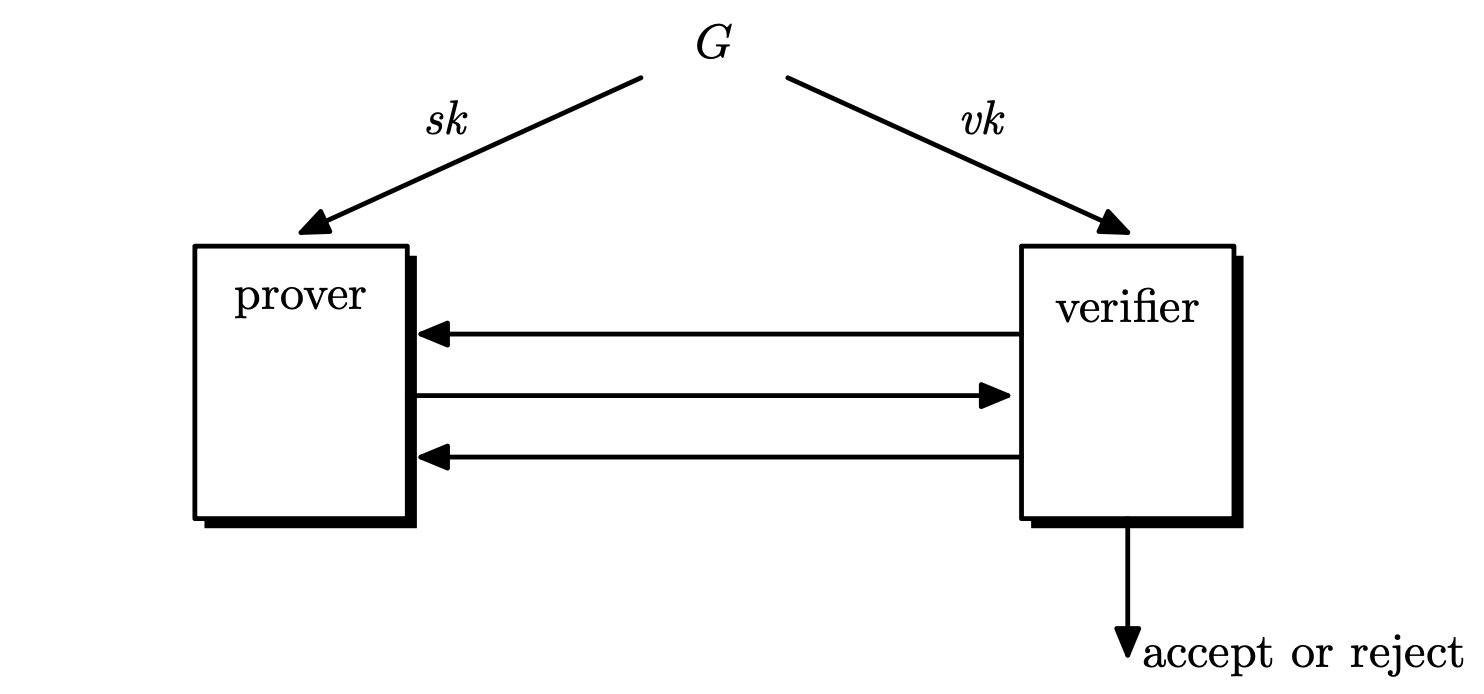
\includegraphics[width=0.6\linewidth]{figures/chapter18/fig1.png}
    \caption{身份认证协议中的证明者与验证者}
    \label{fig:18—1}
\end{figure}

\begin{definition}
一个\textbf{身份识别协议} $\mathcal{I}=(G,P,V)$ 由三部分组成:
\begin{itemize}
    \item $G$ 是一个概率性的\textbf{密钥生成}算法,不接受任何输入,并输出一对密钥 $(vk,sk)$,其中 $vk$ 被称为\textbf{验证密钥 (verification key)},$sk$ 被称为\textbf{私钥 (secret key)};
    \item $P$ 是一个交互式协议算法,被称为\textbf{证明者 (prover)},它接受 $sk$ 作为输入;
    \item $V$ 是一个交互式协议算法,被称为\textbf{验证者 (verifier)},它接受 $vk$ 作为输入,输出 $\mathsf{accept}$ 或 $\mathsf{reject}$。
\end{itemize}
我们要求,当 $P(sk)$ 和 $V(vk)$ 能够正确交互时,$V(vk)$ 总是输出 $\mathsf{accept}$。也就是说,对于 $G$ 的所有可能输出 $(vk,sk)$,如果 $P$ 由 $sk$ 初始化,$V$ 由 $vk$ 初始化,那么当 $P$ 和 $V$ 交互结束时,$V$ 输出 $\mathsf{accept}$ 的概率为 $1$。

\end{definition}